\newpage
\begin{sol}
\begin{enumerate}[label=\textbf{(\alph*)}]
\item The differential equation is once again
$$-\frac{1}{z_0^2}\Psi''+(v(x)-e)\Psi=0$$
with:
$$
v(x) = \begin{cases}
0 &= x<-(2+\gamma) \\
-1 &= -(2+\gamma)<x<-\gamma \\
0 &= -\gamma < x < \gamma \\
-1 &= \gamma < x < 2+\gamma \\
0 &= x > \gamma+2
\end{cases}
$$
Solving this numerically via the Shooting method gives $e=-0.72936$ or $E=-17.26 \text{ eV}$. The wavefunction looks like:
\begin{center}
    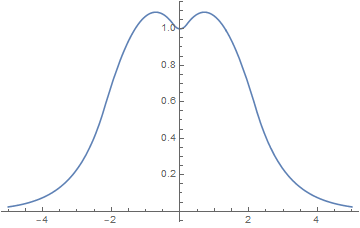
\includegraphics[width=0.4\linewidth]{Images/6-6.png}
\end{center}
\item The energy due to repulsion is $|E_0|=13.6 \text{ eV}$ so the binding energy is:
$$E_b=|E_0|+E=-3.66 \text{ eV}$$
According to Griffiths, the experimentally determined binding energy is $-2.8 \text{ eV}$ so this model is rather accurate.
\end{enumerate}
\end{sol}